Mirko and Slavko are playing with toy animals. First, they choose one of three boards given in the figure below.

Each board consists of cells (shown as circles in the figure) arranged into a one, two or three dimensional grid.

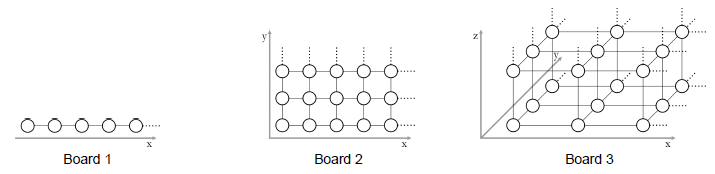
\includegraphics[scale=0.9]{pairs.png}

Mirko then places $N$ little toy animals into the cells.

The distance between two cells is the smallest number of moves that an animal would need in order to reach one cell from the other. In one move, the animal may step into one of the adjacent cells (connected by line segments in the figure).

Two animals can hear each other if the distance between their cells is at most $D$. Slavko's task is to calculate how many pairs of animals there are such that one animal can hear the other.

Write a program that, given the board type, the locations of all animals, and the number $D$, finds the desired number of pairs.